\renewcommand{\tablename}{Tabla}
\chapter{Marcos de Implementación} \label{Chapter:3}

Actualmente hay una gran cantidad de entornos de trabajo desarrollados exclusivamente para el aprendizaje profundo. Algunos de los más populares son TensorFlow, Theano, Caffe, Keras o PyTorch. En el caso particular de este proyecto y tal como se expondrá a lo largo de este capítulo son usados básicamente dos: Keras y Tensorflow, dado que son los más versátiles al ofrecer la mayor cantidad de herramientas que simplifican notablemente las implementaciones y los que permiten una integración más directa con otras plataformas como Google Cloud u OpenCV.

También cabe mencionar que cada uno de estos entornos emplea el lenguaje de programación interpretado Python como interfaz de programación \textit{front end}, lo que lo convierte en el escenario mas extendido para el desarrollo de aplicaciones de aprendizaje automático. Además, Python es capaz de combinarse con lenguajes de programación de bajo nivel como C o C\texttt{++}, que actúan generalmente como \textit{back end}.

\section{Keras y TensorFlow}

Keras es una Interfaz de Programación de Aplicaciones (API) de redes neuronales de alto nivel, escrita en Python y capaz de ejecutarse sobre TensorFlow. Esta última, por su parte, es una biblioteca de software de código abierto desarrollada por el departamento de inteligencia artificial de Google para la computación numérica de alto rendimiento con la capacidad de implementarse y ejecutarse utilizando múltiples Unidades de Procesamiento Central (CPUs), Unidades de Procesamiento Gráfico (GPUs) y Unidades de Procesamiento Tensorial (TPUs).

La decisión del empleo de estas dos herramientas, concretamente de Keras sobre TensorFlow, radica en que su combinación proporciona un entorno modular, extensible y fácil de usar, ofreciendo un gran número de utensilios de aprendizaje profundo. En este contexto, Keras facilita tanto las herramientas para desarrollar las arquitecturas neuronales, como el medio y los métodos para entrenar los modelos. Además, en lo que respecta al campo del reconocimiento visual, pone a disposición de la comunidad una gran variedad de modelos preentrenados con distintas bases de datos y que pueden emplearse para la predicción, la extracción de características y la afinación de otros sistemas que planteen problemas similares. De hecho, la existencia de estos modelos, que son reconocidos como los estados del arte dentro de su ámbito, simplifica notablemente la implementación de técnicas como la transferencia de aprendizaje, tratada en el \autoref{Chapter:TransferLearning}.

\section{Google Cloud Plataform}

Google Cloud Platform es una plataforma que ofrece un conjunto de servicios modulares de computación en la nube, entre los que destacan el almacenamiento de datos, el análisis de datos y el aprendizaje automático. Dentro de este último punto, se van a utilizar básicamente tres herramientas: \begin{itemize}
  \item \textbf{Cloud Machine Learning Engine}. Es un servicio que proporciona un entorno de implementación de modelos complejos de aprendizaje automático, permitiendo ejecutar aplicación desarrolladas sobre TensorFlow con ciertas alteraciones. Concretamente, mediante este servicio es posible realizar tareas previas de procesado de datos, entrenar modelos de aprendizaje profundo y evaluar sistemas existentes.
  
  La GPU empleada por este servicio y la única ofrecida actualmente es la NVIDIA Tesla K80.
  \item \textbf{Compute Engine -- Cloud Datalab}. Este producto permite desarrollar proyectos en máquinas virtuales escalables de alto rendimiento y ejecutarlos en las infraestructuras de Google. El medio específico que se utiliza es Cloud Datalab, que es una herramienta interactiva que posibilita la exploración, el análisis y la visualización de datos, así como el desarrollo de modelos de aprendizaje automático en \textit{notebooks} con Python y TensorFlow.
  
  En este caso se dispone de una GPU más potente, la NVIDIA Tesla P100, que permite superar las limitaciones de memoria impuestas por el servicio Cloud Machine Learning Engine.
  \item \textbf{Cloud Storage}. Es el sistema de almacenamiento de la plataforma Google Cloud. Abarca tareas relacionadas tanto con el suministro, el archivado y el análisis de datos, como con el aprendizaje automático. En este proyecto su utilización se centra en el guardado de los puntos de control de los modelos, así como en el almacenamiento de los registros y métricas que permiten analizar el estado del entrenamiento o del aprendizaje en tiempo real. 
\end{itemize}

\begin{table}
\centering
\begin{tabular}{c|c|c|c|c|}
    \cline{2-5}
    & \textbf{Memoria} & \textbf{Núcleos} & \textbf{\begin{tabular}[c]{@{}c@{}}B/W \\ Memoria\end{tabular}} & \textbf{\begin{tabular}[c]{@{}c@{}}Memoria\\ disponible\end{tabular}} \\ \hline
    \multicolumn{1}{|c|}{\textbf{\begin{tabular}[c]{@{}c@{}}NVIDIA \\ Quadro K4000\end{tabular}}}   & 3 GB GDDR5    & 768 & 134 GB/s    & -- \\ \hline
    \multicolumn{1}{|c|}{\textbf{\begin{tabular}[c]{@{}c@{}}NVIDIA\\ Tesla K80\end{tabular}}}       & 12 GB GDDR5   & 2496 & 240 GB/s   & 1 -- 52 GB \\ \hline
    \multicolumn{1}{|c|}{\textbf{\begin{tabular}[c]{@{}c@{}}NVIDIA\\ Tesla P100\end{tabular}}}      & 16 GB HBM2    & 3584 & 732 GB/s   & 1 -- 104 GB \\ \hline
\end{tabular}
\caption{Comparación entre las GPUs tanteadas durante el desarrollo del proyecto.}
\label{Table:GPU}
\end{table}

El uso de esta plataforma para la afinación de los modelos propuestos en el \autoref{Chapter:5} tiene como finalidad la reducción de forma abrupta del tiempo de aprendizaje. De hecho, empleando las herramientas anteriormente descritas se ha corroborado personalmente un incremento de la velocidad de entrenamiento de entre 6 y 7 veces con respecto a la utilización de un computador con una GPU NVIDIA Quadro K4000 (gama alta del año 2013) y de hasta 30 veces en comparación con el desempeño obtenido por un computador portátil personal que carece de unidades de procesamiento gráfico. Las comparaciones entre estos equipos puede verse en la \autoref{Table:GPU}.

Por último, hace falta mencionar que la elección de Google Cloud Plataform en favor de otros servicio de computación en la nube, como Amazon Web Services o Microsoft Azure, ha estado motivada principalmente por razones económicas y de soporte ya que Google es el proveedor que ofrece la mayor variedad de servicios dentro de su periodo de prueba gratuito.

\section{Bases de Datos}

En el proceso de desarrollo del sistema de reconocimiento de emociones de este proyecto se emplean, directa o indirectamente, tres tipos de bases de datos distintas. Por un lado se hace uso de los conjuntos de datos ImageNet \cite{ImageNet} y VGGFace2 \cite{VGGFace2}, que son precisamente los aprendidos por los modelos preentrenados ofrecidos por Keras. Por el otro destaca FER-2013 \cite{FER-2013}, que es la base de datos mediante la cual se va a realizar el afinamiento de los sistemas iniciales para dotarlos de la capacidad de reconocer expresiones faciales.

\subsection{ImageNet} \label{Chapter:ImageNet}

ImageNet es una base de datos visual enfocada en la investigación de \textit{software} para el reconocimiento de objetos visuales y compuesta por tres subconjuntos de datos: entrenamiento (1.2 millones de imágenes), validación (50\,000 imágenes) y evaluación (100\,000 imágenes). Estas fotografías, recopiladas de Flickr y otros motores de búsqueda, están etiquetadas a mano indicando la presencia o ausencia de 1\,000 categorías de objetos, los cuales abarcan ámbitos tan diversos como razas de perro, especies de plantas u hongos, distintos objetos cotidianos o personas.

Esta amplitud, heterogeneidad y no superposición de clases es la que ha convertido precisamente a ImageNet en el punto de referencia para los algoritmos de clasificación de imágenes, dominados por las redes neuronales convolucionales y las técnicas de aprendizaje profundo desde 2012. Por esta razón, de hecho, gran parte de los modelos que mejor rendimiento han obtenido con esta base de datos se han incluido en la biblioteca de Keras.

\subsection{VGGFace2} \label{Chapter:VGGFace2}

Esta base de datos contiene 3.31 millones de imágenes faciales de 9\,131 sujetos célebres, con un promedio de 362.6 fotografías por individuo y con una gran diversidad de poses, de edades, de iluminación, de etnias y de profesiones. Todo este conjunto de datos se divide en un grupo de entrenamiento de 8\,631 individuos y en uno de pruebas de 500 individuos. Además, VGGFace2 proporciona anotaciones que permiten la evaluación de los distintos sujetos en dos escenarios diferentes: coincidencia de rostros de diferentes posturas y coincidencia de rostros de diferentes edades.

\subsection{FER-2013} \label{Chapter:FER-2013}

\begin{figure}
    \centering
    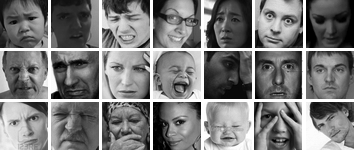
\includegraphics{Images/FER-2013.png}
    \caption{Imágenes extraídas de la base de datos FER-2013 \cite{Pramerdorfer}.}
    \label{fig:FER-2013}
\end{figure}

FER-2013 es la base de datos estáticos de expresiones faciales de mayor relevancia disponible públicamente. Consta de 35\,887 representaciones en escala de grises adquiridas de entornos no acondicionados expresamente con una resolución de $48 \times 48$ píxeles. Este conjunto reúne rostros de distinta naturaleza en términos de edad, orientación de la cara, etnia y género, tal y como puede observase en la \autoref{fig:FER-2013} y está dividido en tres subgrupos: entrenamiento, validación y evaluación con 28\,709, 3\,589 y 3\,589 muestras respectivamente. Asimismo, cada una de las imágenes está etiquetada con respecto a la expresión manifestada por el sujeto en la fotografía.

\begin{table}
\centering
\begin{tabular}{c|c|c|c|c|c|c|c|}
    \cline{2-8}
    & \textbf{Ira} & \textbf{Asco} & \textbf{Miedo} & \textbf{Alegría} & \textbf{Tristeza} & \textbf{Sorpresa} & \textbf{Neutral} \\ \hline
    \multicolumn{1}{|c|}{\textbf{\begin{tabular}[c]{@{}c@{}}Núm. de\\ imágenes\end{tabular}}} & 4\,953 & 547 & 5\,121 & 8\,989 & 6\,077 & 4\,002 & 6\,198 \\ \hline
\end{tabular}
\caption{Número de imágenes por cada expresión facial de la base de datos FER-2013.}
\label{Table:FER-2013}
\end{table}

En la \autoref{Table:FER-2013} se muestra la cantidad de imágenes en esta base de datos de las seis expresiones básicas y la expresión neutral. Como puede advertirse, hay un desequilibrio de clases notable, hecho que va a influir negativamente en el desempeño del modelo, especialmente para las emociones con menor representación. Como solución parcial a este problema se plantean en la \autoref{Chapter:DataAugmentation} una serie de técnicas de aumento de datos.

Por último, cabe destacar que la precisión humana sobre este conjunto es de aproximadamente $65\pm 5\%$ \cite{FER-2013_human_acc}.

\section{OpenCV} \label{Chapter:OpenCV}

OpenCV es una librería de código abierto de visión por computador escrita en C\slash C\texttt{++} y con un fuerte enfoque en aplicaciones en tiempo real. Por este motivo y teniendo en cuenta su extendido uso, es la que se va a utilizar para el desarrollo del software encargado de detectar y capturar el rostro de forma periódica y en pseudo tiempo real para la posterior identificación de la expresión facial o, dicho de otra forma, para la confección del espejo inteligente. Las características y la descripción detallada de los algoritmos empleados para tal fin se exponen en la \autoref{Chapter:FaceDetection}.

Por su parte, la implementación de este sistema se va a llevar a cabo mediante Python y, dado que OpenCV fue diseñada para ser efectiva computacionalmente, en un sistema operativo GNU/Linux optimizado para el hardware de la Raspberry PI.
